\documentclass[tikz,border=8pt]{standalone}
\usepackage{amsmath}
\usetikzlibrary{positioning, arrows.meta, calc}

\begin{document}

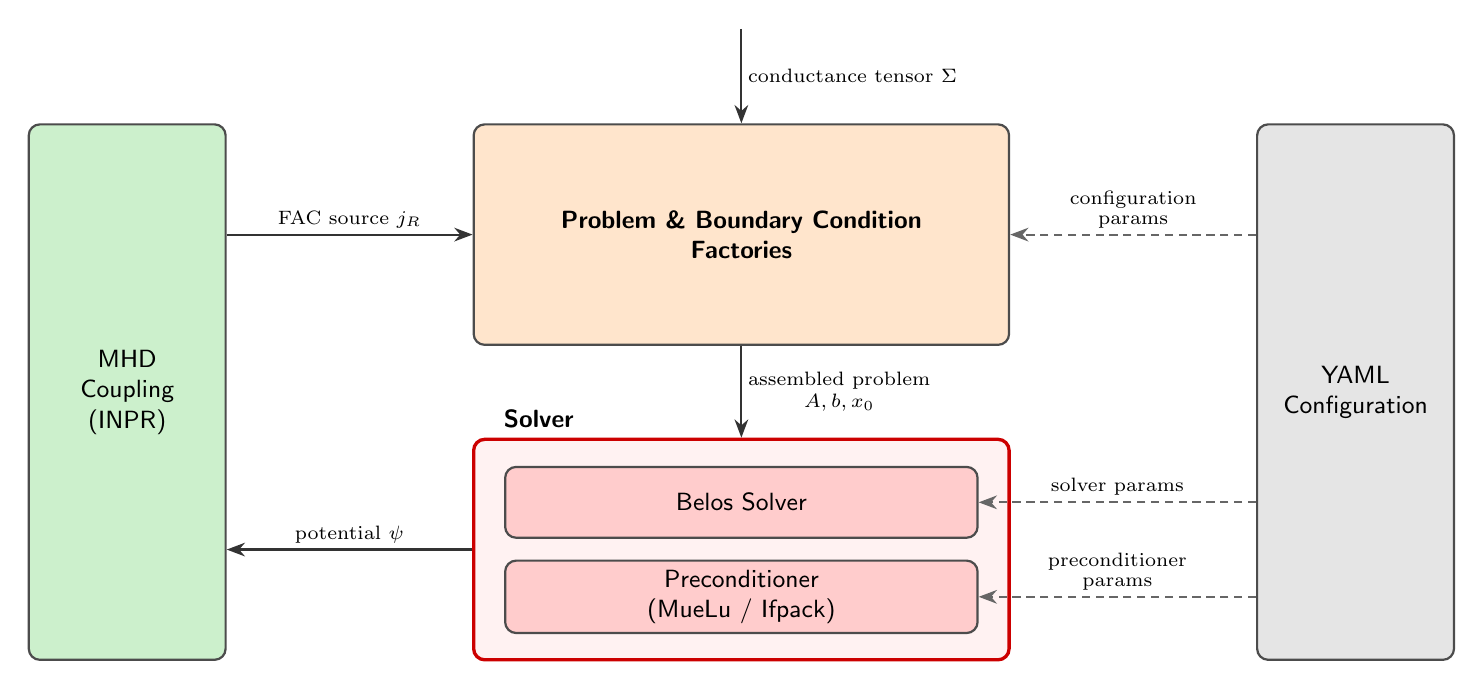
\begin{tikzpicture}[
		>=Stealth,
		% Standard composite box style (fixed size to ensure exact stacking)
		compbox/.style 2 args={
				rectangle, rounded corners, draw=#1!80!black, very thick,
				fill=#1!5, minimum width=6.8cm, minimum height=2.8cm,
				label={[anchor=south west, font=\sffamily\small\bfseries, xshift=8pt, yshift=0pt]north west:#2}
			},
		% Inner sub-boxes
		subbox/.style={
				rectangle, rounded corners, draw=black!70, thick,
				fill=#1!20, minimum width=6.0cm, minimum height=0.9cm,
				font=\sffamily\small, align=center
			},
		% Standard standalone blocks
		stdbox/.style={
				rectangle, rounded corners, draw=black!70, thick,
				fill=#1!20, font=\sffamily\small, align=center
			},
		% Arrows
		arrowdata/.style={->, thick, draw=black!80},
		arrowparam/.style={->, densely dashed, thick, draw=black!60},
		labarrow/.style={font=\scriptsize, fill=white, inner sep=2pt, align=center}
	]

	% ==========================================
	% 1. MAIN VERTICAL STACK (X=0)
	% ==========================================
	% Shifted up to center the diagram. Factories are now the top-most visible block.

	% Block 1: Factories (Y=2.0)
	\node[stdbox=orange, minimum width=6.8cm, minimum height=2.8cm, font=\sffamily\small\bfseries]
	(factories) at (0, 2.0) {Problem \& Boundary Condition\\Factories};

	% Block 2: Solver (Y=-2.0)
	\node[compbox={red}{Solver}] (solver) at (0, -2.0) {};
	\node[subbox=red] (belos) at ([yshift=0.6cm]solver.center) {Belos Solver};
	\node[subbox=red] (prec) at ([yshift=-0.6cm]solver.center) {Preconditioner\\(MueLu / Ifpack)};


	% ==========================================
	% 2. MHD COUPLING (LEFT, X=-7.8)
	% ==========================================
	% Width = 2.5cm, height = 6.8cm, centered vertically with the stack.

	\node[stdbox=green!70!black, minimum width=2.5cm, minimum height=6.8cm]
	(inpr) at (-7.8, 0.0) {MHD\\Coupling\\(INPR)};


	% ==========================================
	% 3. YAML CONFIGURATION (RIGHT, X=7.8)
	% ==========================================
	% Height adjusted to 6.8cm to perfectly match the visible Factories+Solver stack.
	% Center moved to Y=0.0 to guarantee perfect alignment.

	\node[stdbox=gray, minimum width=2.5cm, minimum height=6.8cm]
	(yaml) at (7.8, 0.0) {YAML\\Configuration};


	% ==========================================
	% 4. DATA FLOW ARROWS (SOLID)
	% ==========================================

	% New: Input arrow leading in from above (where Conductivity Model used to be)
	\draw[arrowdata] ([yshift=1.2cm]factories.north) -- node[labarrow, right] {conductance tensor $\Sigma$} (factories.north);

	% Main pipeline flow
	\draw[arrowdata] (factories.south) -- node[labarrow, right] {assembled problem\\$A, b, x_0$} (solver.north);

	% Horizontal MHD Integration
	\draw[arrowdata] (inpr.east |- factories.west) -- node[labarrow, above] {FAC source $j_R$} (factories.west);
	\draw[arrowdata] (solver.west) -- node[labarrow, above] {potential $\psi$} (inpr.east |- solver.west);


	% ==========================================
	% 5. PARAMETER FLOW ARROWS (DASHED)
	% ==========================================

	% YAML parameter lines routed cleanly from the gray block.

	% Into Factories
	\draw[arrowparam] (yaml.west |- factories.east) -- node[labarrow, above] {configuration\\[-0.3ex]params} (factories.east);

	% Into Solver sub-boxes
	\draw[arrowparam] (yaml.west |- belos.east) -- node[labarrow, above] {solver params} (belos.east);
	\draw[arrowparam] (yaml.west |- prec.east) -- node[labarrow, above] {preconditioner\\[-0.3ex]params} (prec.east);

\end{tikzpicture}

\end{document}
